\section{Cubedate: Secure Low-Power Continuous Deployment for CubeSat Software}
\label{sec:low-power-orbital-communication-arch}

The process we use for securing ThingSat software udpates (Cubedate) is decomposed in six phases shown \autoref{fig:phases}. 

\subsection{Basic software life-cycle phases}

During a preliminary, pre-flight phase (\textit{Phase 0}) the authorized maintainer for the CubeSat-hosted payload
produces and flashes the payload with commissioning material:
a bootloader, the initial firmware, and authorized crypto material (a public key, and a crypographically strong hash function).
Once the hosted payload is commissioned it can be sent to the CubeSat operator of installation in the CubeSat.


Once the CubeSat in orbit, the hosted payload maintainer can trigger iterations through cycles of Phases 1-5, whereby
the authorized maintainer can build a new software update (\textit{Phase 1}), hash the update
and sign the hash (\textit{Phase 2}) then push a network transfer (PUT) towards the hosted payload via the ground station and the OBC. The next time it wakes up, the hosted payload can
then ping and fetch (GET) the update from the OBC (\textit{Phase 3}), proceed to verify the signature and the hash (\textit{Phase 4}),
and upon successful verification, install/boot the new software (\textit{Phase 5}), otherwise the update is dropped.

\begin{figure}[t]
    \centering
    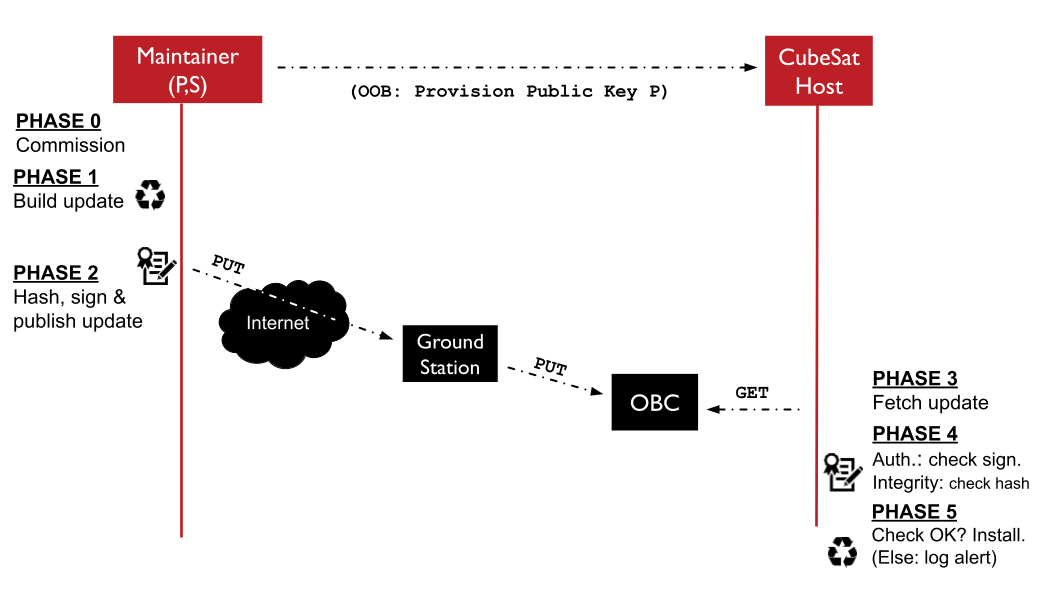
\includegraphics[width=0.5\textwidth]{Figures/CubeSat-Payload-update.png}
    \caption{CubeSat hosted payload secure software update process.}
    \label{fig:phases}
\end{figure}

\subsection{Requirements}

\paragraph*{communication protocols}
\paragraph*{software/firmware updates}
\paragraph*{software/configuration updates requirements}

\subsection{Architecture}
\subsubsection{OS}: RIOT
\subsubsection{Network Stack}: COAP/LibCSP/CAN
\subsubsection{Mission Workflow}: mission files
\subsubsection{DevOps Workflow}: SUIT + containers
\paragraph*{SUIT}
\paragraph*{Containerization}

